\documentclass{beamer}
\usetheme{Madrid}
\usecolortheme{beaver}
\usepackage{color}
\usepackage{graphicx}
\usepackage[utf8]{inputenc}
\usepackage{tikz}
\usetikzlibrary{shapes.misc}


\newcommand{\bi}{\begin{itemize}}
\newcommand{\ei}{\end{itemize}}

%Information to be included in the title page:
\title[Regularization and CNNs]{String Theory meets Machine Learning\\
	- Regularization and CNNs}
\author{Robin Schneider}
\institute{Uppsala University}
\date{November 2020}


\begin{document}
	
	\frame{\titlepage}



\begin{frame}
\frametitle{Learning Hodge numbers}
A physics problem
\bi
\item There are 7890 distinct Complete Intersection Calabi Yau manifolds
\item Described by configuration matrices
\begin{align}
\mathcal{M} =  \left[
\begin{array}{c||ccc}
n_0 & p^0_1 & \cdots & p^0_{K} \\
\vdots & \vdots & \ddots & \vdots \\
n_r & p^{r}_1 & \cdots & p^{r}_K  \\
\end{array}
\right]^{h^{(1,1)},h^{(2,1)}}_{\chi}.
\end{align}
\item Want to learn Hodge numbers. We use a fully connected neural network for that.
\ei
\end{frame}

\begin{frame}
\frametitle{Dense NN and CICYlist}
\begin{figure}[t]
	\begin{minipage}{0.5\linewidth}
		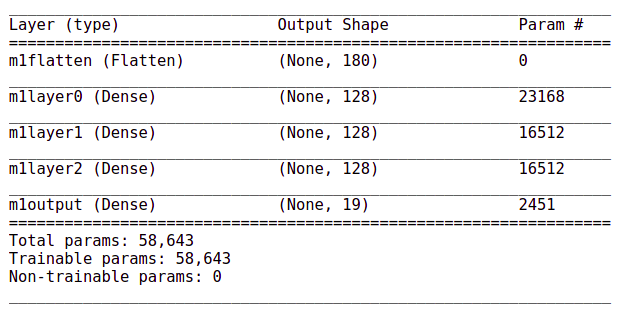
\includegraphics[scale=0.28]{dense.png}
	\end{minipage}
	\begin{minipage}{0.45\linewidth}
		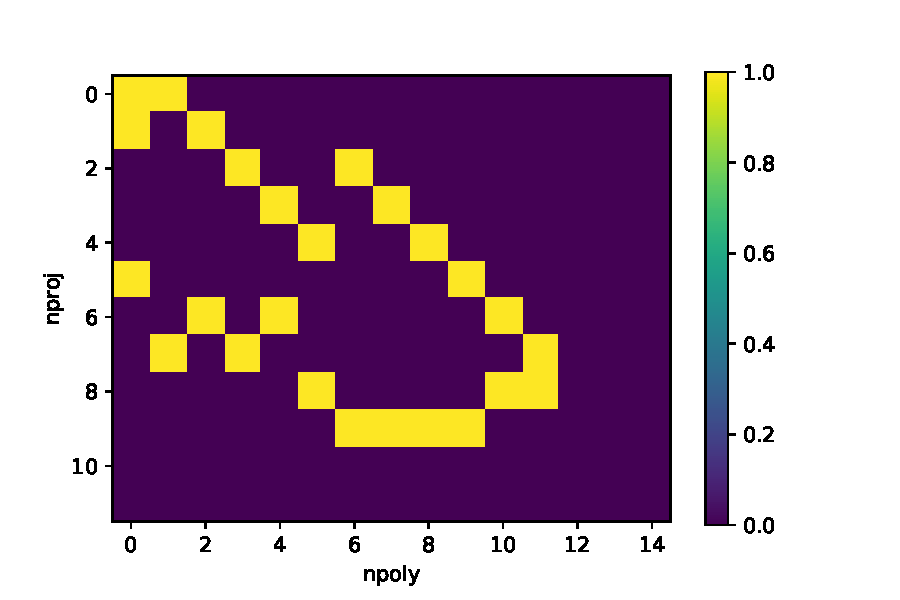
\includegraphics[scale=0.4]{cicy150.pdf}
	\end{minipage}
	\caption{\it On the left fully connected NN and on the right CICY with index 150 visualized as a 2d image.}
	\label{fig:cicy}
\end{figure}
\end{frame}
	
\begin{frame}
\frametitle{Overfitting, low bias high variance}
\begin{figure}
\centering
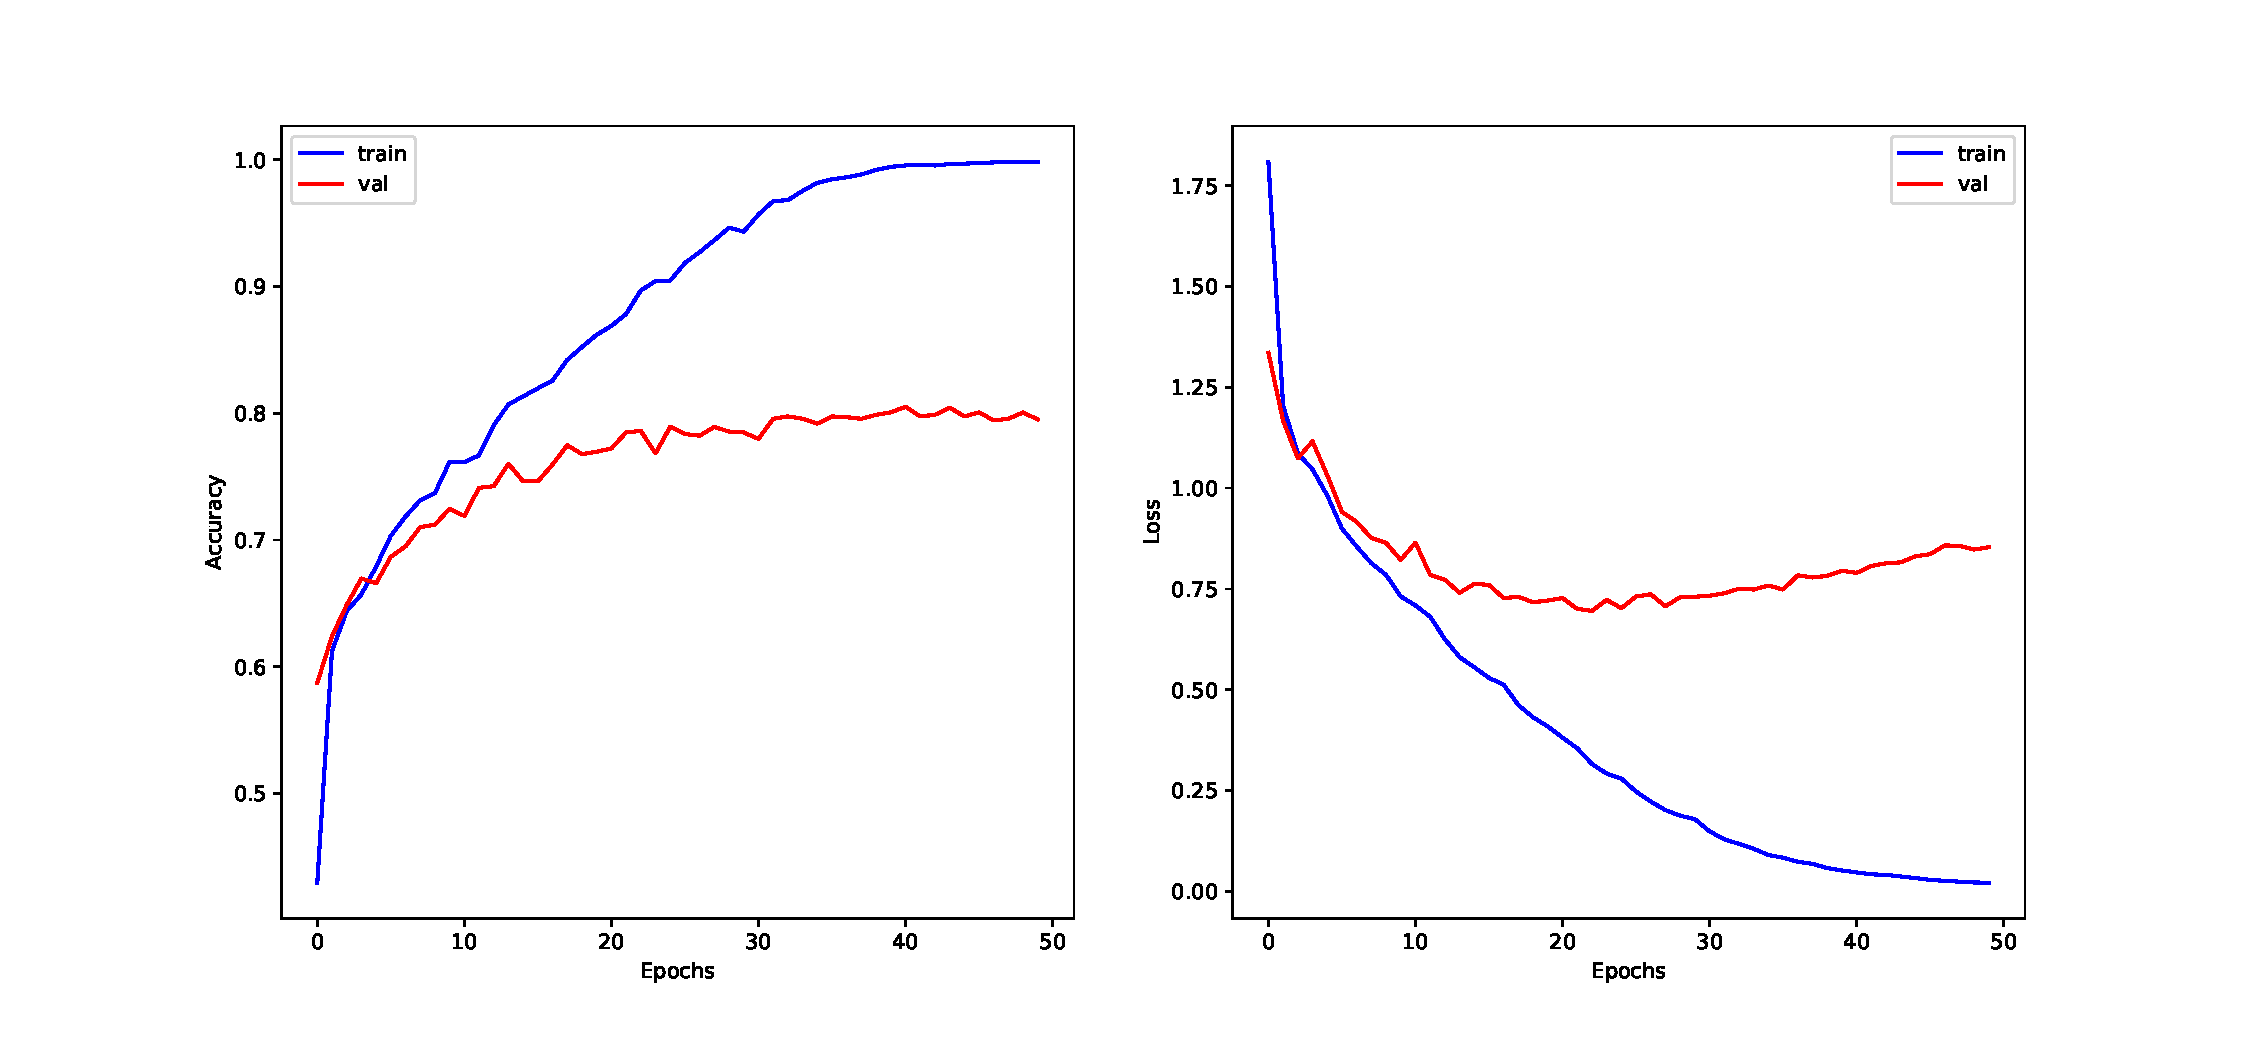
\includegraphics[scale=0.33]{cicy_no_reg.pdf}
\caption{ \it Loss and accuracy plot of a fully connected NN learning $h^{1,1}$ of CICYs.}
\end{figure}
\end{frame}


\begin{frame}
\frametitle{Bias and Variance}
Assume the true data of our model follows
\begin{align}
y = f(x; \theta) + \epsilon \qquad \text{ with } \epsilon \sim \mathcal{N}(0, \sigma^2_\epsilon).
\end{align}

\textbf{Bias:} $\mathbb{E}_{D} [f(x;\hat{\theta}_D)] - f(x;\theta)$.

\textbf{Variance:} $\mathbb{E}_D[(f(x;\hat{\theta}_D) - \mathbb{E}_D[f(x;\hat{\theta}_D)])^2]$

What does the expected error look like?
\pause
\begin{align}
\mathbb{E}_{D,\epsilon} [J] &= \mathbb{E}_{D,\epsilon} \left[ \sum_{i=1}^n (y_i - f(x_i; \hat{\theta}_D))^2 \right] \nonumber \\
& = \sum_i^n \bigg[ \underbrace{\sigma^2_\epsilon}_{\text{Noise}} + \underbrace{(\mathbb{E}_D[f(x_i; \hat{\theta}_D)]-f(x_i; \theta) )^2}_{\text{Bias}^2} + \nonumber \\
& \qquad\qquad \qquad   \underbrace{\mathbb{E}_D[(f(x_i; \hat{\theta}_D) - \mathbb{E}_D[f(x_i; \hat{\theta}_D)])^2 ]}_{\text{Variance}} \bigg]
\end{align}
\end{frame}

\begin{frame}
\frametitle{Bias and Variance tradeoff}
\begin{figure}
	\centering
	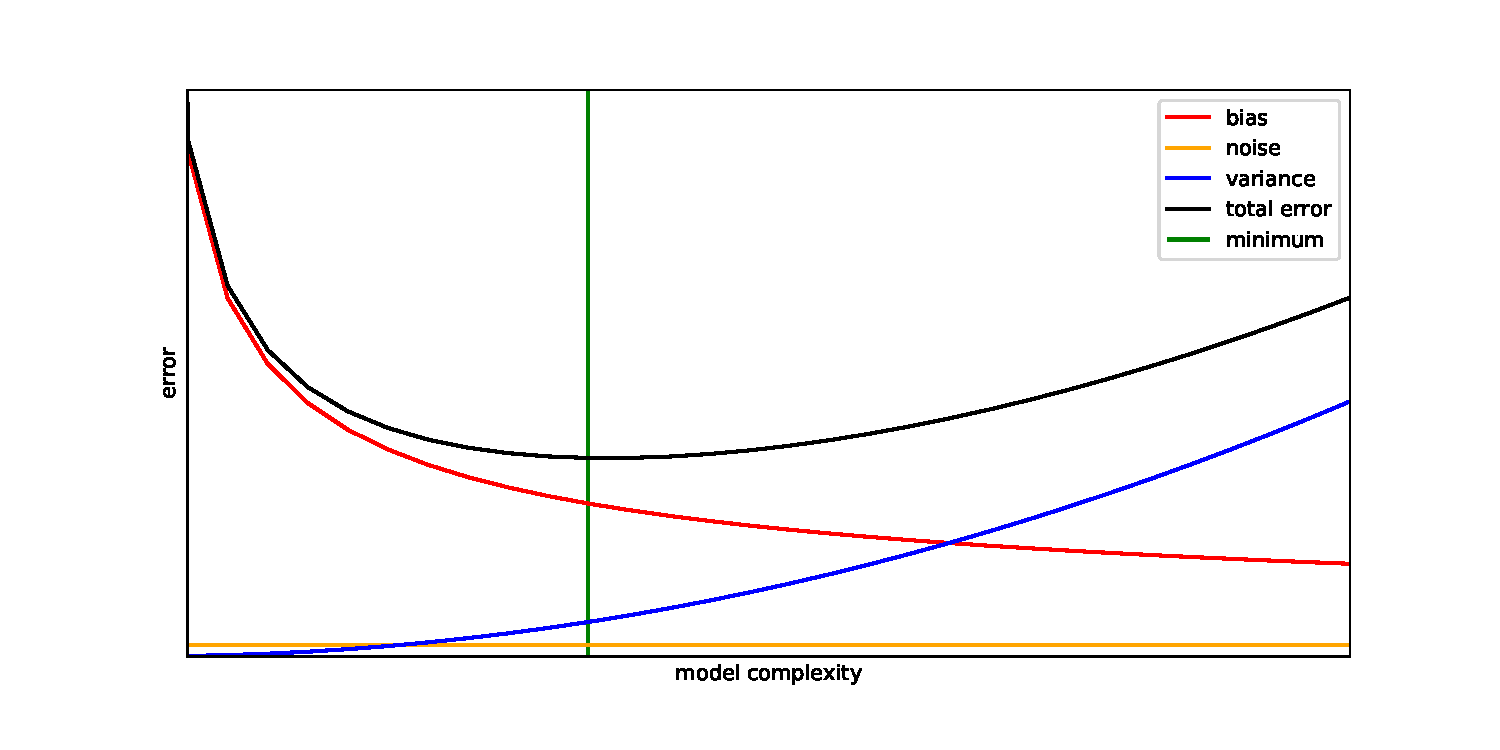
\includegraphics[scale=0.5]{bias_variance.pdf}
	\caption{ \it Model error and its decomposition as model complexity grows.}
\end{figure}
\end{frame}


%\begin{frame}
%\frametitle{Bias Variance tradeoff}
%The tradeoff:
%\bi
%\item Test error can be decomposed into bias and variance.
%\item Increase complexity of our model (more parameters), decreases Bias, but increases Variance.
%\item A low Bias model requires more training data.
%\item With little training data use less complex (high bias) model.
%\item High bias model might underfit the training data.
%\item High bias models have the advantage, that they are more efficiently %trained.
%\ei
%\end{frame}

\begin{frame}
\frametitle{Regularization}
How to decrease overfitting? \pause

Introduce \textbf{regularization}. Simplest way is to add penalty term to cost function
\begin{align}
J_{\text{total}}(\theta) = J_{\text{reg}}(\theta) + \lambda J_{\text{penalty}} (\theta) .
\end{align}
Usually the penalty term takes the form
\begin{align}
J_{\text{penalty}} (\theta) = \frac{1}{2} \sum_i |\theta_i|^q.
\end{align}
\end{frame}


\begin{frame}
\frametitle{L2 - Ridge, weight decay}
$q = 2$: L2 (LASSO, weight decay) regression. 

Assume Gaussian prior $p(\theta) = \mathcal{N}(\theta|0, \alpha^{-1})$ and likelihood with precision parameter $\beta^{-1}$. Then maximize with respect to log posterior (recall Bayes theorem: $p(\theta | D) \propto p(D|\theta) p ( \theta)$):
\begin{align}
\hat{\theta} & = \underset{\theta}{\arg \max} (\log (p(D|\theta) p(\theta)))
\end{align}
\pause
which results in the following loss
\begin{align}
J(\theta) = \frac{\beta}{2} \sum_{i=1}^{n} (f(x_n; \theta) - y_n)^2 + \frac{\alpha}{2} \theta^2
\end{align}
such that $\lambda = \frac{\alpha}{\beta}$. One can solve this and finds that each component shrinks by $\hat{\theta}^{L2} = \frac{d_j^2}{d_j^2 + \lambda} \hat{\theta}^{LS}$.
\end{frame}

\begin{frame}
\frametitle{L1 - LASSO, sparse}

$q = 1$: L1 (LASSO, Sparse) regularization with loss function
\begin{align}
J(\theta) = \frac{1}{2} \sum_{i=1}^{n} (f(x_n; \theta) -y_n)^2 + \frac{\lambda}{2} |\theta|
\end{align}
is equivalent to linear regression with the additional condition
\begin{align}
	&\hat{\theta} = \underset{\theta}{\arg \min} ((f(x; \theta) - y)^2)  \text{ and }  \lambda \geq  |\theta|
\end{align}
We can't solve this exactly.
\pause
However assuming $x$ is orthogonal one can analyze it using subgradient methods to find
\begin{align}
	\hat{\theta}^{LASSO} = \text{sign}(\hat{\theta}^{LS}) (|\hat{\theta}^{LS}| - \lambda)_+ 
\end{align}
$\hat{\theta}^{LS}$ optimal least square fit value. The subscript $+$ denotes positive part. Thus $\lambda$ determines a threshold which sets small parameters to zero.
\end{frame}


\begin{frame}
\frametitle{L1 and L2 in a picture}
\begin{figure}
	\centering
	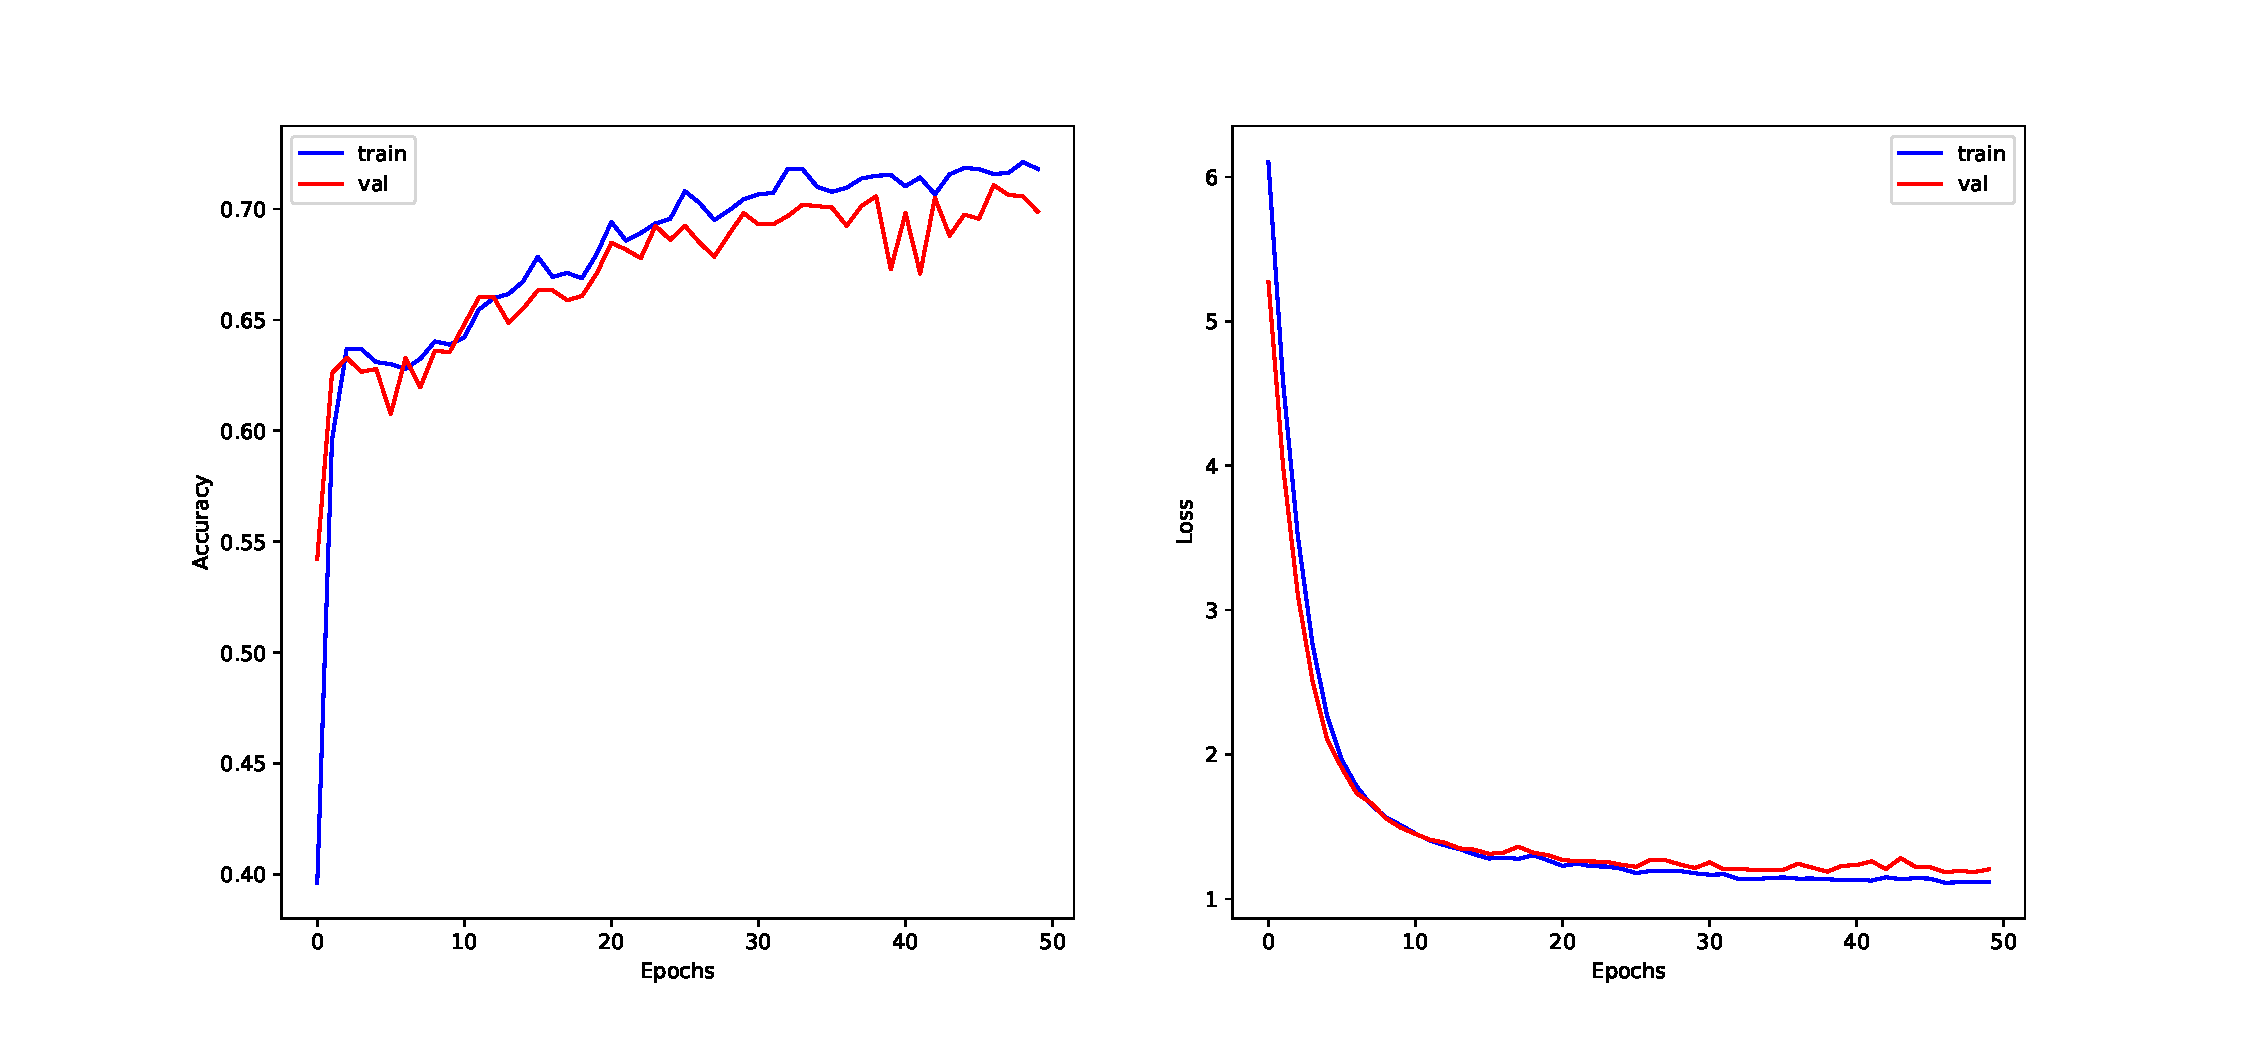
\includegraphics[scale=0.33]{cicy_l1l2_reg.pdf}
	\caption{ \it Accuracy and loss plot of a fully connected neural network learning $h^{1,1}$ of CICYs with l1, l2 values of $(0.001,0.001)$.}
\end{figure}
\end{frame}

\begin{frame}
\frametitle{Dropout}
\begin{figure}[t]
	\centering
	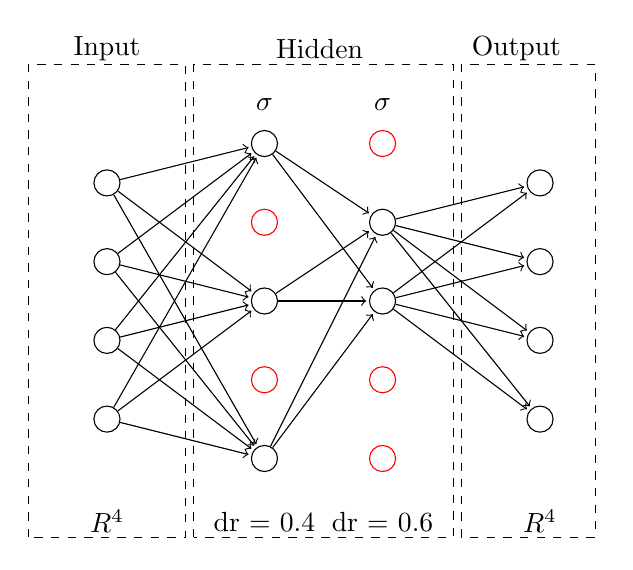
\begin{tikzpicture}[shorten >=1pt,node distance=2cm,auto]
	\tikzset{
		annot/.style={
			text width=4em,
			text centered,		
		}
	}
	\tikzset{%
		every neuron/.style={
			circle,
			draw,
		},
		neuron missing/.style={
			draw=red,
			circle,
			draw,
		},
	}
	
	% Frames
	\draw[dashed] (0,0) rectangle (2,6);
	\draw[dashed] (2.1,0) rectangle (5.4,6);
	\draw[dashed] (5.5,0) rectangle (7.2,6);
	
	% Neuron Nodes
	% Input
	\foreach \m/\l [count=\y] in {1,2,3,4}
	\node [every neuron/.try, neuron \m/.try] (I-\m) at (1,5.5-\y) {};%
	\node [annot] (Input) at (1,6.2) {Input};%
	\node [annot] (IR) at (1,0.2) {$\mathbb{R}^{4}$};%
	
	%H1
	\foreach \m/\l [count=\y] in {1,missing,2,missing,3}
	\node [every neuron/.try, neuron \m/.try] (H1-\m) at (3,6-\y) {};
	\node [annot] (H1a) at (3,5.5) {$\sigma$};%
	\node [annot] (H1R) at (3,0.2) {dr = $0.4$};%
	
	%H2
	\foreach \m/\l [count=\y] in {missing,1,2,missing,missing}
	\node [every neuron/.try, neuron \m/.try] (H2-\m) at (4.5,6-\y) {};%
	\node [annot] (H2a) at (4.5,5.5) {$\sigma$};%
	\node [annot] (H2R) at (4.5,0.2) {dr = $0.6$};%
	\node [annot] (Hidden) at (3.7,6.2) {Hidden};	
	
	%O1
	\foreach \m/\l [count=\y] in {1,2,3,4}
	\node [every neuron/.try, neuron \m/.try] (O1-\m) at (6.5,5.5-\y) {};%
	\node [annot] (O2R) at (6.5,0.2) {$\mathbb{R}^{4}$};%
	%\node [annot] (O2l) at (11.5,6) {Value};%
	\node [annot] (Output) at (6.2,6.2) {Output};		
	
	% Connecting lines
	\foreach \i in {1,2,3,4}
	\foreach \j in {1,...,3}
	\draw [->] (I-\i) -- (H1-\j);
	\foreach \i in {1,...,3}
	\foreach \j in {1,...,2}
	\draw [->] (H1-\i) -- (H2-\j);
	\foreach \i in {1,...,2}
	\foreach \j in {1,2,3,4}
	\draw [->] (H2-\i) -- (O1-\j);
	\end{tikzpicture}
	\caption{\it A fully connected Neural Network of a classification problem. In red dropped nodes during training.}
	\label{NNclass}
\end{figure}
\end{frame}

\begin{frame}
\frametitle{Dropout in a picture}
\begin{figure}
	\centering
	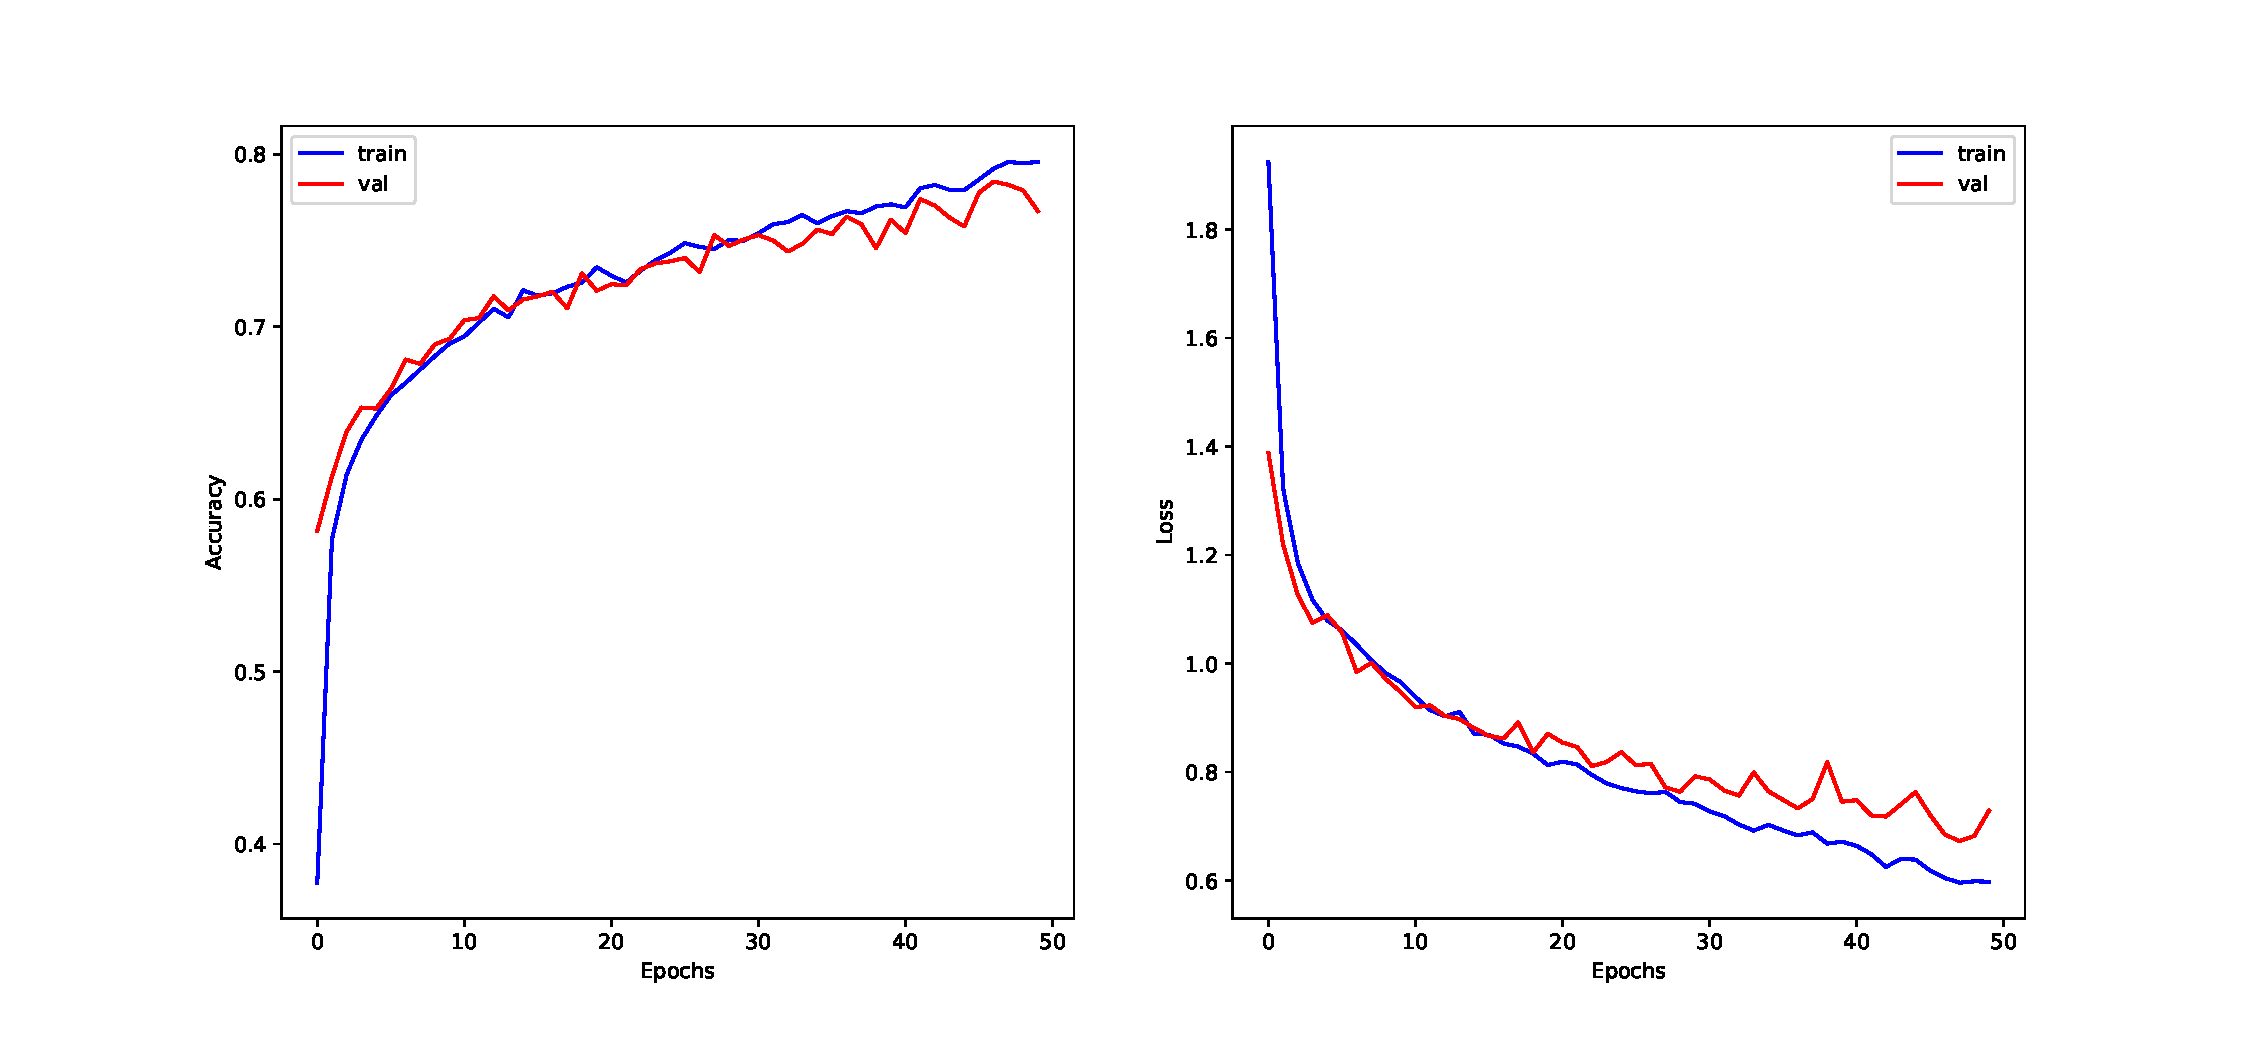
\includegraphics[scale=0.33]{cicy_dropout.pdf}
	\caption{\it Accuracy and loss plot of a fully connected neural network learning $h^{1,1}$ of CICYs with a dropout rate of $0.2$.}
\end{figure}
\end{frame}

\begin{frame}
\frametitle{Convolutional Neural Networks}

CNNs gained wide popularity with the publishing of AlexNET which won the ImageNet competition in 2012
\begin{itemize}
	\item Higher accuracy (less prone to overfitting; AlexNET had $>10\%$ accuracy over runner up)
	\item less parameters (e.g. 3mio weights for single dense neuron in 1000x1000px)
	\item More natural (learns features and filters of the image)
\end{itemize}
\end{frame}

\begin{frame}
\frametitle{CNN}
\begin{center}
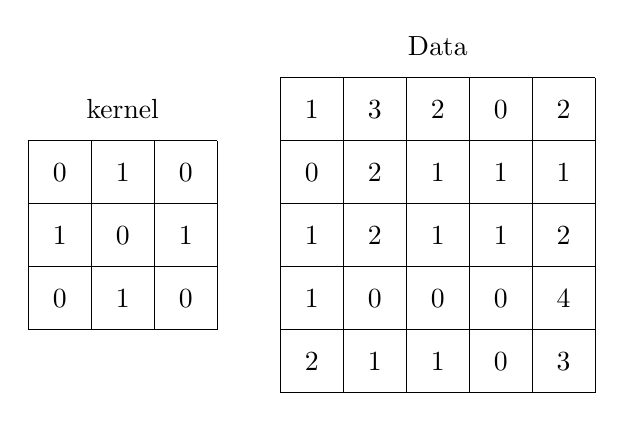
\begin{tikzpicture}[scale=0.8]
	% Boxes
	\draw[solid] (0,0) grid (3,3);
	\draw[solid] (4,-1) grid (9,4);
	
	% kernel
	\node (k1) at (0.5,0.5) {0};
	\node (k2) at (0.5,1.5) {1};
	\node (k3) at (0.5,2.5) {0};
	\node (k4) at (1.5,0.5) {1};
	\node (k5) at (1.5,1.5) {0};
	\node (k6) at (1.5,2.5) {1};
	\node (k7) at (2.5,0.5) {0};
	\node (k8) at (2.5,1.5) {1};
	\node (k9) at (2.5,2.5) {0};
	\node (kh) at (1.5,3.5) {kernel};
	
	%image
	\node (i1) at (4.5,-0.5) {2};
	\node (i2) at (4.5,0.5) {1};
	\node (i3) at (4.5,1.5) {1};
	\node (i4) at (4.5,2.5) {0};
	\node (i5) at (4.5,3.5) {1};
	\node (i6) at (5.5,-0.5) {1};
	\node (i7) at (5.5,0.5) {0};
	\node (i8) at (5.5,1.5) {2};
	\node (i9) at (5.5,2.5) {2};
	\node (i10) at (5.5,3.5) {3};
	\node (i11) at (6.5,-0.5) {1};
	\node (i12) at (6.5,0.5) {0};
	\node (i13) at (6.5,1.5) {1};
	\node (i14) at (6.5,2.5) {1};
	\node (i15) at (6.5,3.5) {2};
	\node (i16) at (7.5,-0.5) {0};
	\node (i17) at (7.5,0.5) {0};
	\node (i18) at (7.5,1.5) {1};
	\node (i19) at (7.5,2.5) {1};
	\node (i20) at (7.5,3.5) {0};
	\node (i21) at (8.5,-0.5) {3};
	\node (i22) at (8.5,0.5) {4};
	\node (i23) at (8.5,1.5) {2};
	\node (i24) at (8.5,2.5) {1};
	\node (i25) at (8.5,3.5) {2};
	\node (i25) at (6.5,4.5) {Data};
	
		%\foreach \x [count=\i] in {0,-3,2}
	%	\foreach \y [count=\j] in {1,1,-1}
	%		\node (k-\i-\j) at (-0.5+\i,-0.5+\j) {{\x+\y}};
\end{tikzpicture}
\end{center}
\bi
\item First, define kernel shape
\item Depth is the number of kernels scanning over the data
\item Stride is the scan length
\item Padding is number of zeros cols/rows added to the boundaries
\ei
\end{frame}

\begin{frame}
\frametitle{CNN}
\begin{center}
	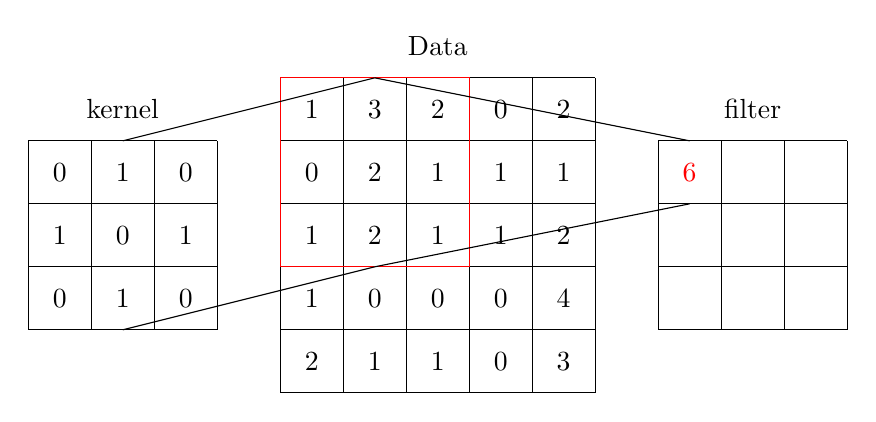
\begin{tikzpicture}[scale=0.8]
	% Boxes
	\draw[solid] (0,0) grid (3,3);
	\draw[solid] (4,-1) grid (9,4);
	\draw[solid] (10,0) grid (13,3);
	
	% the other boxes
	\draw[solid, color=red] (4,1) rectangle (7,4);
	\node (f) at (11.5, 3.5) {filter};
	\draw[-] (1.5,0) -- (5.5,1);
	\draw[-] (1.5,3) -- (5.5,4);
	\draw[-] (5.5,1) -- (10.5,2);
	\draw[-] (5.5,4) -- (10.5,3);

	
	
	% kernel
	\node (k1) at (0.5,0.5) {0};
	\node (k2) at (0.5,1.5) {1};
	\node (k3) at (0.5,2.5) {0};
	\node (k4) at (1.5,0.5) {1};
	\node (k5) at (1.5,1.5) {0};
	\node (k6) at (1.5,2.5) {1};
	\node (k7) at (2.5,0.5) {0};
	\node (k8) at (2.5,1.5) {1};
	\node (k9) at (2.5,2.5) {0};
	\node (kh) at (1.5,3.5) {kernel};
	
	%image
	\node (i1) at (4.5,-0.5) {2};
	\node (i2) at (4.5,0.5) {1};
	\node (i3) at (4.5,1.5) {1};
	\node (i4) at (4.5,2.5) {0};
	\node (i5) at (4.5,3.5) {1};
	\node (i6) at (5.5,-0.5) {1};
	\node (i7) at (5.5,0.5) {0};
	\node (i8) at (5.5,1.5) {2};
	\node (i9) at (5.5,2.5) {2};
	\node (i10) at (5.5,3.5) {3};
	\node (i11) at (6.5,-0.5) {1};
	\node (i12) at (6.5,0.5) {0};
	\node (i13) at (6.5,1.5) {1};
	\node (i14) at (6.5,2.5) {1};
	\node (i15) at (6.5,3.5) {2};
	\node (i16) at (7.5,-0.5) {0};
	\node (i17) at (7.5,0.5) {0};
	\node (i18) at (7.5,1.5) {1};
	\node (i19) at (7.5,2.5) {1};
	\node (i20) at (7.5,3.5) {0};
	\node (i21) at (8.5,-0.5) {3};
	\node (i22) at (8.5,0.5) {4};
	\node (i23) at (8.5,1.5) {2};
	\node (i24) at (8.5,2.5) {1};
	\node (i25) at (8.5,3.5) {2};
	\node (i25) at (6.5,4.5) {Data};

\pause
	\node[red] (f1) at (10.5,2.5) {6};	
	\end{tikzpicture}
\end{center}
\end{frame}

\begin{frame}
\frametitle{CNN}
\begin{center}
	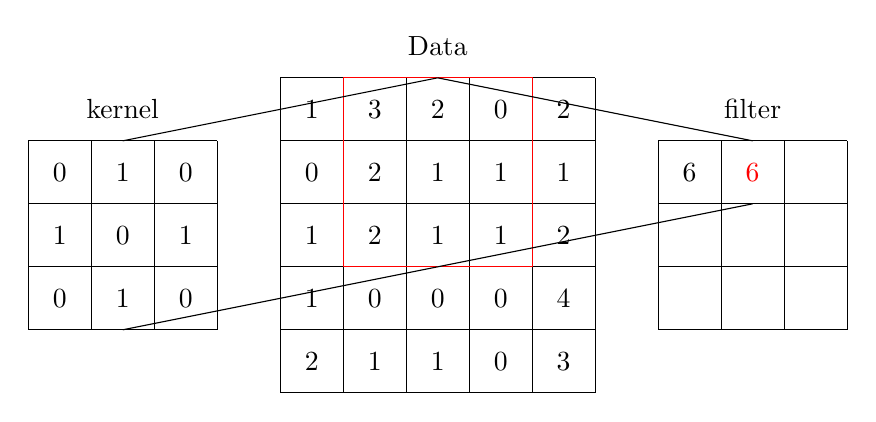
\begin{tikzpicture}[scale=0.8]
	% Boxes
	\draw[solid] (0,0) grid (3,3);
	\draw[solid] (4,-1) grid (9,4);
	\draw[solid] (10,0) grid (13,3);
	
	% the other boxes
	\draw[solid, color=red] (5,1) rectangle (8,4);
	\draw[-] (1.5,0) -- (6.5,1);
	\draw[-] (1.5,3) -- (6.5,4);
	\draw[-] (6.5,1) -- (11.5,2);
	\draw[-] (6.5,4) -- (11.5,3);
	
	\node (f) at (11.5, 3.5) {filter};
	\node (f1) at (10.5,2.5) {6};	
	
	% kernel
	\node (k1) at (0.5,0.5) {0};
	\node (k2) at (0.5,1.5) {1};
	\node (k3) at (0.5,2.5) {0};
	\node (k4) at (1.5,0.5) {1};
	\node (k5) at (1.5,1.5) {0};
	\node (k6) at (1.5,2.5) {1};
	\node (k7) at (2.5,0.5) {0};
	\node (k8) at (2.5,1.5) {1};
	\node (k9) at (2.5,2.5) {0};
	\node (kh) at (1.5,3.5) {kernel};
	
	%image
	\node (i1) at (4.5,-0.5) {2};
	\node (i2) at (4.5,0.5) {1};
	\node (i3) at (4.5,1.5) {1};
	\node (i4) at (4.5,2.5) {0};
	\node (i5) at (4.5,3.5) {1};
	\node (i6) at (5.5,-0.5) {1};
	\node (i7) at (5.5,0.5) {0};
	\node (i8) at (5.5,1.5) {2};
	\node (i9) at (5.5,2.5) {2};
	\node (i10) at (5.5,3.5) {3};
	\node (i11) at (6.5,-0.5) {1};
	\node (i12) at (6.5,0.5) {0};
	\node (i13) at (6.5,1.5) {1};
	\node (i14) at (6.5,2.5) {1};
	\node (i15) at (6.5,3.5) {2};
	\node (i16) at (7.5,-0.5) {0};
	\node (i17) at (7.5,0.5) {0};
	\node (i18) at (7.5,1.5) {1};
	\node (i19) at (7.5,2.5) {1};
	\node (i20) at (7.5,3.5) {0};
	\node (i21) at (8.5,-0.5) {3};
	\node (i22) at (8.5,0.5) {4};
	\node (i23) at (8.5,1.5) {2};
	\node (i24) at (8.5,2.5) {1};
	\node (i25) at (8.5,3.5) {2};
	\node (i25) at (6.5,4.5) {Data};
\pause
	\node[red] (f2) at (11.5,2.5) {6};

	\end{tikzpicture}
\end{center}
\end{frame}

\begin{frame}
\frametitle{CNN}
\begin{center}
	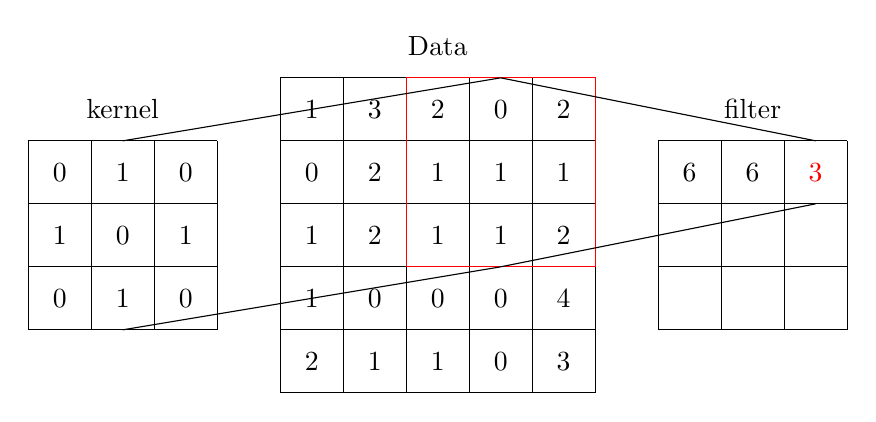
\begin{tikzpicture}[scale=0.8]
	% Boxes
	\draw[solid] (0,0) grid (3,3);
	\draw[solid] (4,-1) grid (9,4);
	\draw[solid] (10,0) grid (13,3);
	
	% the other boxes
	\draw[solid, color=red] (6,1) rectangle (9,4);
	\draw[-] (1.5,0) -- (7.5,1);
	\draw[-] (1.5,3) -- (7.5,4);
	\draw[-] (7.5,1) -- (12.5,2);
	\draw[-] (7.5,4) -- (12.5,3);
	
	\node (f) at (11.5, 3.5) {filter};
	\node (f1) at (10.5,2.5) {6};
	\node (f2) at (11.5,2.5) {6};
	\node[red] (f3) at (12.5,2.5) {3};
	
	
	% kernel
	\node (k1) at (0.5,0.5) {0};
	\node (k2) at (0.5,1.5) {1};
	\node (k3) at (0.5,2.5) {0};
	\node (k4) at (1.5,0.5) {1};
	\node (k5) at (1.5,1.5) {0};
	\node (k6) at (1.5,2.5) {1};
	\node (k7) at (2.5,0.5) {0};
	\node (k8) at (2.5,1.5) {1};
	\node (k9) at (2.5,2.5) {0};
	\node (kh) at (1.5,3.5) {kernel};
	
	%image
	\node (i1) at (4.5,-0.5) {2};
	\node (i2) at (4.5,0.5) {1};
	\node (i3) at (4.5,1.5) {1};
	\node (i4) at (4.5,2.5) {0};
	\node (i5) at (4.5,3.5) {1};
	\node (i6) at (5.5,-0.5) {1};
	\node (i7) at (5.5,0.5) {0};
	\node (i8) at (5.5,1.5) {2};
	\node (i9) at (5.5,2.5) {2};
	\node (i10) at (5.5,3.5) {3};
	\node (i11) at (6.5,-0.5) {1};
	\node (i12) at (6.5,0.5) {0};
	\node (i13) at (6.5,1.5) {1};
	\node (i14) at (6.5,2.5) {1};
	\node (i15) at (6.5,3.5) {2};
	\node (i16) at (7.5,-0.5) {0};
	\node (i17) at (7.5,0.5) {0};
	\node (i18) at (7.5,1.5) {1};
	\node (i19) at (7.5,2.5) {1};
	\node (i20) at (7.5,3.5) {0};
	\node (i21) at (8.5,-0.5) {3};
	\node (i22) at (8.5,0.5) {4};
	\node (i23) at (8.5,1.5) {2};
	\node (i24) at (8.5,2.5) {1};
	\node (i25) at (8.5,3.5) {2};
	\node (i25) at (6.5,4.5) {Data};
	
	\end{tikzpicture}
\end{center}
\end{frame}

\begin{frame}
\frametitle{CNN}
\begin{center}
	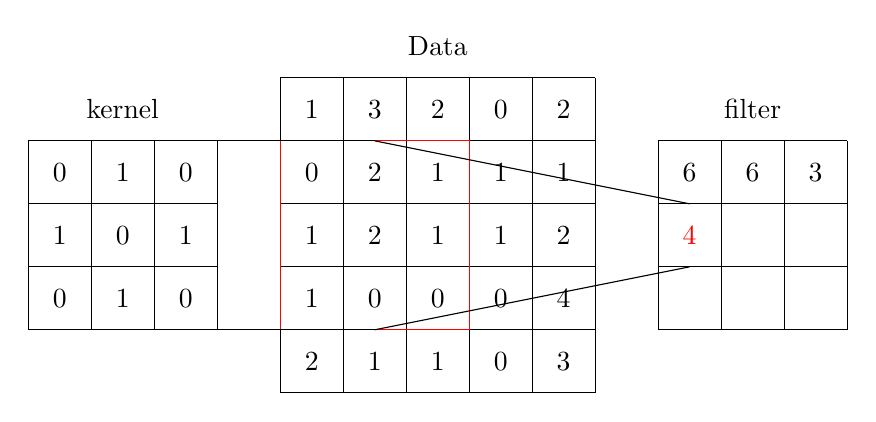
\begin{tikzpicture}[scale=0.8]
	% Boxes
	\draw[solid] (0,0) grid (3,3);
	\draw[solid] (4,-1) grid (9,4);
	\draw[solid] (10,0) grid (13,3);
	
	% the other boxes
	\draw[solid, color=red] (4,0) rectangle (7,3);
	\draw[-] (1.5,0) -- (5.5,0);
	\draw[-] (1.5,3) -- (5.5,3);
	\draw[-] (5.5,0) -- (10.5,1);
	\draw[-] (5.5,3) -- (10.5,2);
	
	\node (f) at (11.5, 3.5) {filter};
	\node (f1) at (10.5,2.5) {6};
	\node (f2) at (11.5,2.5) {6};
	\node (f3) at (12.5,2.5) {3};
	
	
	% kernel
	\node (k1) at (0.5,0.5) {0};
	\node (k2) at (0.5,1.5) {1};
	\node (k3) at (0.5,2.5) {0};
	\node (k4) at (1.5,0.5) {1};
	\node (k5) at (1.5,1.5) {0};
	\node (k6) at (1.5,2.5) {1};
	\node (k7) at (2.5,0.5) {0};
	\node (k8) at (2.5,1.5) {1};
	\node (k9) at (2.5,2.5) {0};
	\node (kh) at (1.5,3.5) {kernel};
	
	%image
	\node (i1) at (4.5,-0.5) {2};
	\node (i2) at (4.5,0.5) {1};
	\node (i3) at (4.5,1.5) {1};
	\node (i4) at (4.5,2.5) {0};
	\node (i5) at (4.5,3.5) {1};
	\node (i6) at (5.5,-0.5) {1};
	\node (i7) at (5.5,0.5) {0};
	\node (i8) at (5.5,1.5) {2};
	\node (i9) at (5.5,2.5) {2};
	\node (i10) at (5.5,3.5) {3};
	\node (i11) at (6.5,-0.5) {1};
	\node (i12) at (6.5,0.5) {0};
	\node (i13) at (6.5,1.5) {1};
	\node (i14) at (6.5,2.5) {1};
	\node (i15) at (6.5,3.5) {2};
	\node (i16) at (7.5,-0.5) {0};
	\node (i17) at (7.5,0.5) {0};
	\node (i18) at (7.5,1.5) {1};
	\node (i19) at (7.5,2.5) {1};
	\node (i20) at (7.5,3.5) {0};
	\node (i21) at (8.5,-0.5) {3};
	\node (i22) at (8.5,0.5) {4};
	\node (i23) at (8.5,1.5) {2};
	\node (i24) at (8.5,2.5) {1};
	\node (i25) at (8.5,3.5) {2};
	\node (i25) at (6.5,4.5) {Data};	
\pause
	\node[red] (f4) at (10.5,1.5) {4};

	\end{tikzpicture}
\end{center}
\end{frame}

\begin{frame}
\frametitle{CNN}
\begin{center}
	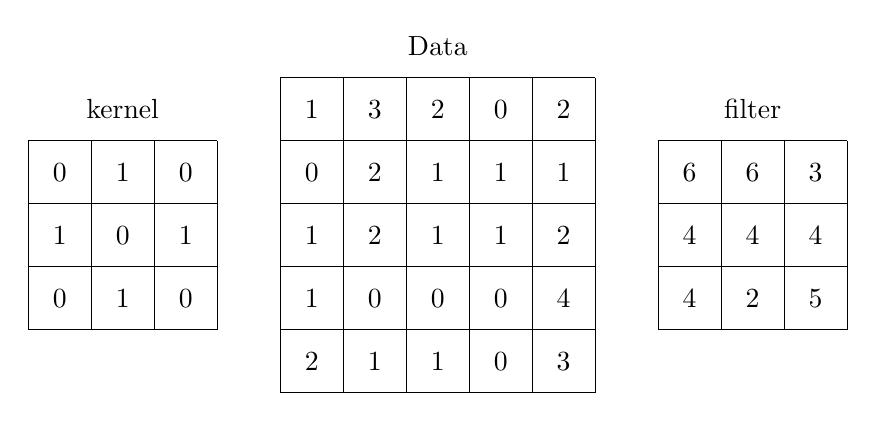
\begin{tikzpicture}[scale=0.8]
	% Boxes
	\draw[solid] (0,0) grid (3,3);
	\draw[solid] (4,-1) grid (9,4);
	\draw[solid] (10,0) grid (13,3);
	
	% the other boxes
	%\draw[solid, color=red] (4,0) rectangle (7,3);
	%\draw[-] (1.5,0) -- (6.5,-1);
	%\draw[-] (1.5,3) -- (5.5,3);
	%\draw[-] (5.5,0) -- (10.5,1);
	%\draw[-] (5.5,3) -- (10.5,2);
	
	\node (f) at (11.5, 3.5) {filter};
	\node (f1) at (10.5,2.5) {6};
	\node (f2) at (11.5,2.5) {6};
	\node (f3) at (12.5,2.5) {3};
	\node (f4) at (10.5,1.5) {4};
	\node (f5) at (11.5,1.5) {4};
	\node (f6) at (12.5,1.5) {4};
	\node (f7) at (10.5,0.5) {4};
	\node (f8) at (11.5,0.5) {2};
	\node (f9) at (12.5,0.5) {5};
	
	% kernel
	\node (k1) at (0.5,0.5) {0};
	\node (k2) at (0.5,1.5) {1};
	\node (k3) at (0.5,2.5) {0};
	\node (k4) at (1.5,0.5) {1};
	\node (k5) at (1.5,1.5) {0};
	\node (k6) at (1.5,2.5) {1};
	\node (k7) at (2.5,0.5) {0};
	\node (k8) at (2.5,1.5) {1};
	\node (k9) at (2.5,2.5) {0};
	\node (kh) at (1.5,3.5) {kernel};
	
	%image
	\node (i1) at (4.5,-0.5) {2};
	\node (i2) at (4.5,0.5) {1};
	\node (i3) at (4.5,1.5) {1};
	\node (i4) at (4.5,2.5) {0};
	\node (i5) at (4.5,3.5) {1};
	\node (i6) at (5.5,-0.5) {1};
	\node (i7) at (5.5,0.5) {0};
	\node (i8) at (5.5,1.5) {2};
	\node (i9) at (5.5,2.5) {2};
	\node (i10) at (5.5,3.5) {3};
	\node (i11) at (6.5,-0.5) {1};
	\node (i12) at (6.5,0.5) {0};
	\node (i13) at (6.5,1.5) {1};
	\node (i14) at (6.5,2.5) {1};
	\node (i15) at (6.5,3.5) {2};
	\node (i16) at (7.5,-0.5) {0};
	\node (i17) at (7.5,0.5) {0};
	\node (i18) at (7.5,1.5) {1};
	\node (i19) at (7.5,2.5) {1};
	\node (i20) at (7.5,3.5) {0};
	\node (i21) at (8.5,-0.5) {3};
	\node (i22) at (8.5,0.5) {4};
	\node (i23) at (8.5,1.5) {2};
	\node (i24) at (8.5,2.5) {1};
	\node (i25) at (8.5,3.5) {2};
	\node (i25) at (6.5,4.5) {Data};	
	\end{tikzpicture}
\end{center}
\end{frame}

\begin{frame}
\frametitle{Pooling}
Variations:
\bi
\item Max pooling - returns max value
\item Average pooling - returns mean value
\ei
Similar to convolutional blocks:
\bi
\item Define, pooling size.
\item Define, stride length.
\item Define, padding.
\ei
\pause
Advantages:
\bi
\item Reduces dimension
\item Preserves translational invariance
\ei
\end{frame}


\begin{frame}
\frametitle{CNN + Pooling}
\begin{figure}
\begin{center}
	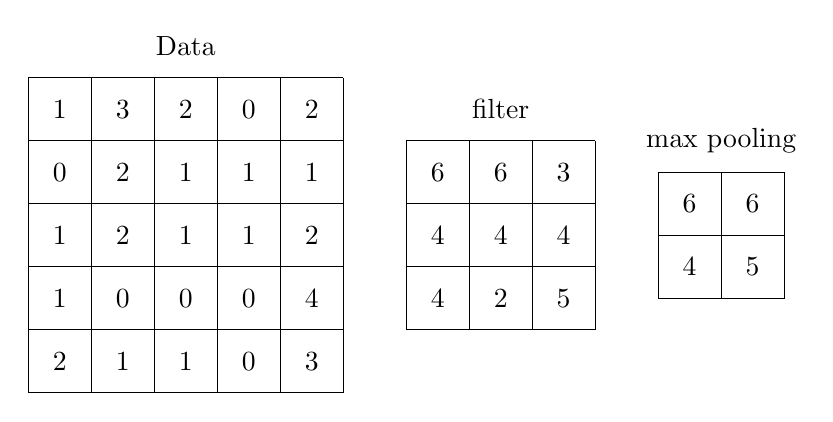
\begin{tikzpicture}[scale=0.8]
	% Boxes
	\draw[solid] (4,-1) grid (9,4);
	\draw[solid] (10,0) grid (13,3);
	\draw[solid] (14,0.5) rectangle (16,2.5);

	\draw[solid] (15,0.5) rectangle (15,2.5);
	\draw[solid] (14,1.5) rectangle (16,1.5);

	\node (p) at (15, 3) {max pooling};
	
	
	\node (f) at (11.5, 3.5) {filter};
	\node (f1) at (10.5,2.5) {6};
	\node (f2) at (11.5,2.5) {6};
	\node (f3) at (12.5,2.5) {3};
	\node (f4) at (10.5,1.5) {4};
	\node (f5) at (11.5,1.5) {4};
	\node (f6) at (12.5,1.5) {4};
	\node (f7) at (10.5,0.5) {4};
	\node (f8) at (11.5,0.5) {2};
	\node (f9) at (12.5,0.5) {5};
	
	
	%image
	\node (i1) at (4.5,-0.5) {2};
	\node (i2) at (4.5,0.5) {1};
	\node (i3) at (4.5,1.5) {1};
	\node (i4) at (4.5,2.5) {0};
	\node (i5) at (4.5,3.5) {1};
	\node (i6) at (5.5,-0.5) {1};
	\node (i7) at (5.5,0.5) {0};
	\node (i8) at (5.5,1.5) {2};
	\node (i9) at (5.5,2.5) {2};
	\node (i10) at (5.5,3.5) {3};
	\node (i11) at (6.5,-0.5) {1};
	\node (i12) at (6.5,0.5) {0};
	\node (i13) at (6.5,1.5) {1};
	\node (i14) at (6.5,2.5) {1};
	\node (i15) at (6.5,3.5) {2};
	\node (i16) at (7.5,-0.5) {0};
	\node (i17) at (7.5,0.5) {0};
	\node (i18) at (7.5,1.5) {1};
	\node (i19) at (7.5,2.5) {1};
	\node (i20) at (7.5,3.5) {0};
	\node (i21) at (8.5,-0.5) {3};
	\node (i22) at (8.5,0.5) {4};
	\node (i23) at (8.5,1.5) {2};
	\node (i24) at (8.5,2.5) {1};
	\node (i25) at (8.5,3.5) {2};
	\node (i25) at (6.5,4.5) {Data};	
\pause
\node (p1) at (14.5,2) {6};
\node (p2) at (14.5,1) {4};
\node (p3) at (15.5,2) {6};
\node (p4) at (15.5,1) {5};
	\end{tikzpicture}
\end{center}
\caption{\it Combined 3x3 convolutional kernel and 2x2 max pooling with zero padding and stride of one.}
\end{figure}
\end{frame}

%\begin{frame}
%\frametitle{What do the filters learn?}
%Add more MNIST digits filter learning. Picture.
%\end{frame}

\begin{frame}
\frametitle{Inception Architectures}
GoogleNet {\color{blue}[1409.4842]} state of the art algorithm in 2014 at ImageNet. Utilizes Inception blocks:
\begin{itemize}
	\item Have several convolutional blocks with different kernels in parallel 	\item Concatenate results
	\pause 
	\item (Optional) Use pooling
	\item (Optional) Use batch normalization {\color{blue} [1502.03167]}, such that mean activation is about 0 and variance close to 1:
	\begin{align}
		\hat{x}^k = \frac{x^k - \mu^k_B}{\sqrt{(\sigma^k_B)^2 + \epsilon}}
	\end{align}
	Then transform
	\begin{align}
		y^k = \gamma^k\hat{x}^k + \beta^k
	\end{align}
\end{itemize}
\end{frame}

\begin{frame}
\frametitle{Inception Block}
\begin{figure}
	\centering
	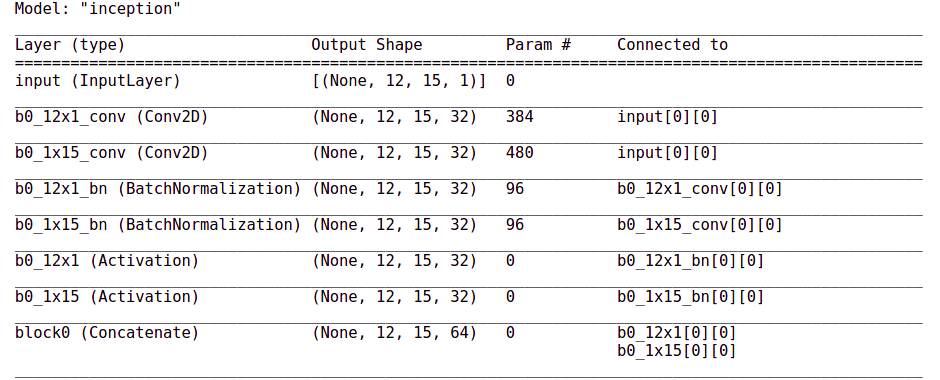
\includegraphics[scale=0.28]{inception_block.png}
	\caption{\it Inception block applied to learning CICY hodge numbers.}
\end{figure}
\end{frame}

\begin{frame}
\frametitle{GoogleNet}
\begin{figure}
	\centering
	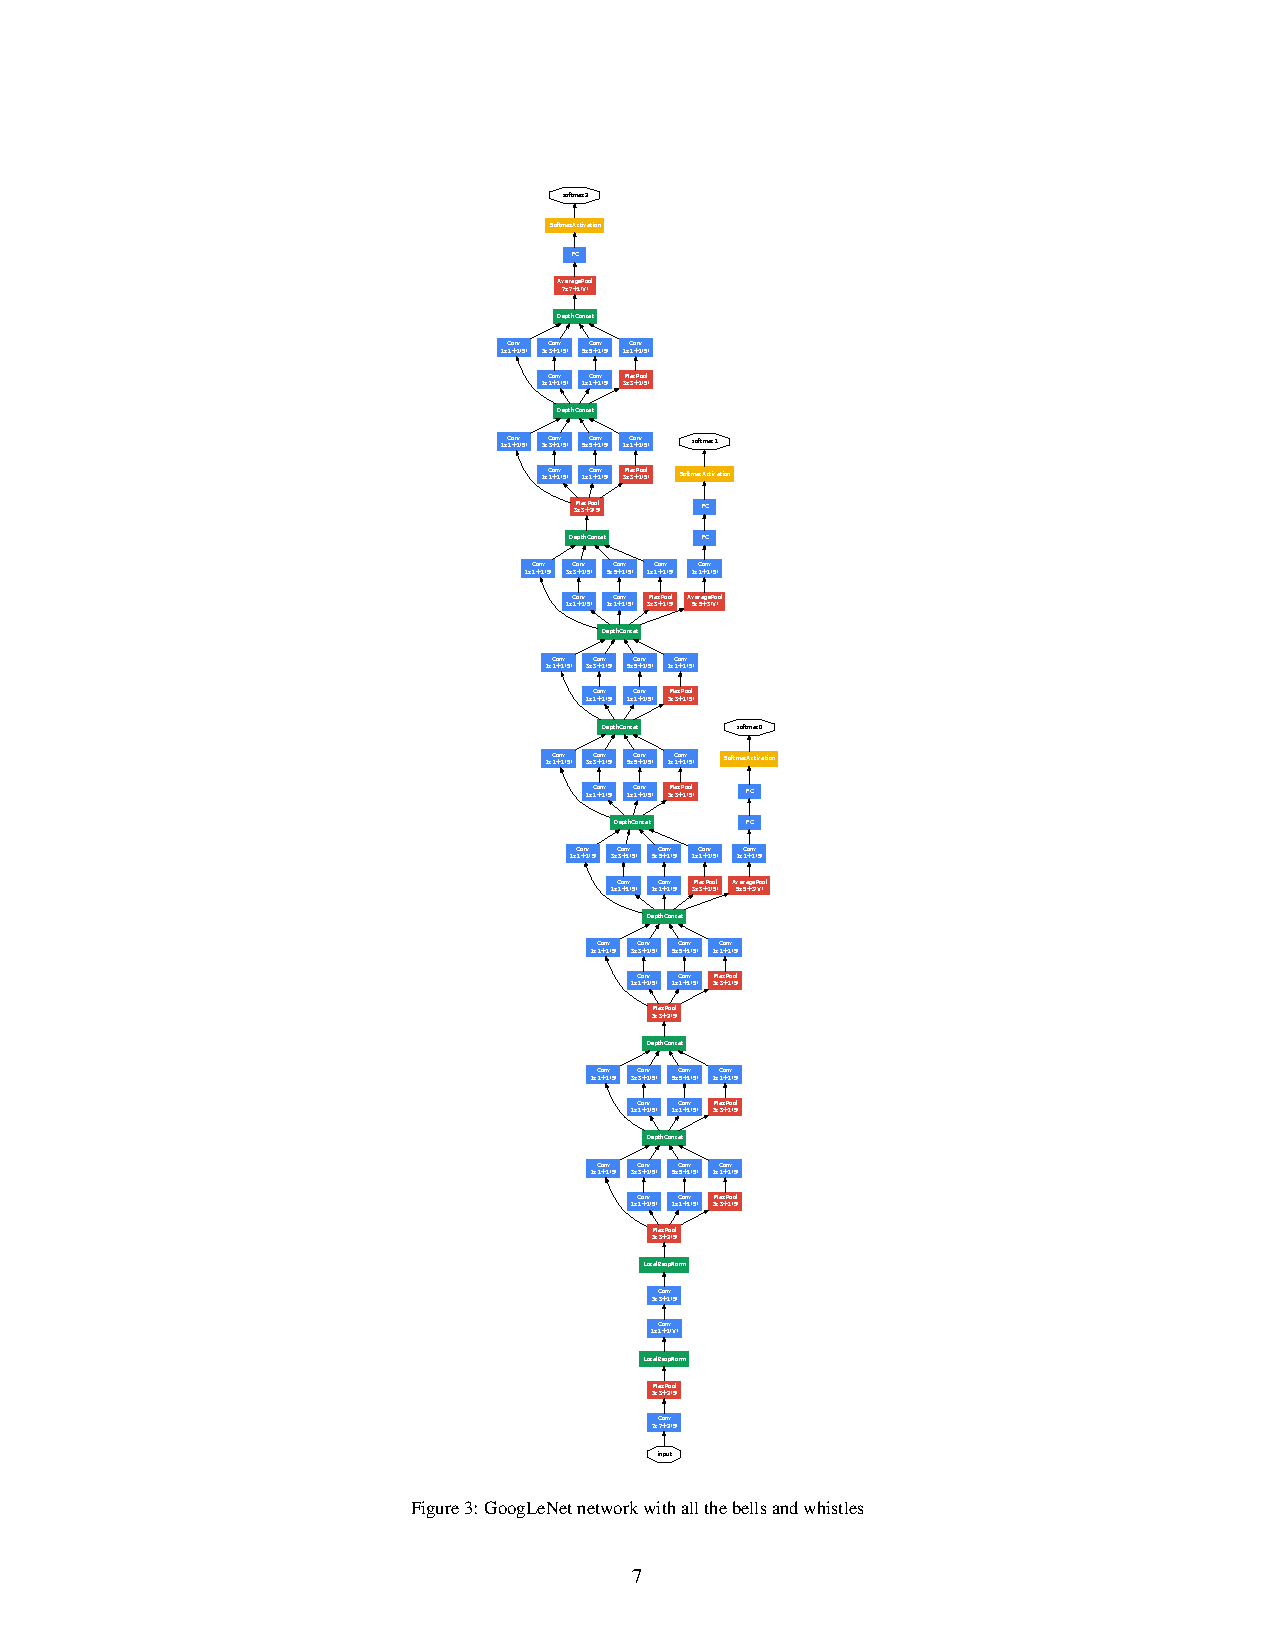
\includegraphics[scale=0.28]{googlenet.pdf}
\end{figure}
\end{frame}

\begin{frame}
\frametitle{Application: Learning Hodge numbers}
Reproduce some results of the early literature. We will predict Hodge numbers of Complete Intersection Calabi Yau 3-folds
\begin{itemize}
	\item Kernel methods and dense NN by He et al. {\color{blue}[1706.02714,1806.03121,1903.03113]}
	\item Using Inception architecture by Erbin and Finotello {\color{blue}[2007.13379]}
	\item Recently four folds were investigated by He and Lukas {\color{blue}[2009.02544]}
\end{itemize}
\end{frame}

\end{document}